% Chapter Template

\chapter{Implementing the PO-TITE-CRM trial design into ADePT-DDR} % Main chapter title

\label{Chapter2} % For referencing this chapter elsewhere, use \ref{Chapter2}

%----------------------------------------------------------------------------------------
%	SECTION 1
%----------------------------------------------------------------------------------------

\section{Introduction}

Worldwide there are approximately 600,000 new cases of Head and Neck Squamous Cell Carcinoma (HNSCC) each year \cite{stranskyMutationalLandscapeHead2011}. Of which, 12,000 occur in the UK with the most common forms of treatment being surgery, radiotherapy and/or chemotherapy \cite{cancerreaserchukHeadNeckCancers2017}. Radiotherapy is essential for the treatment of cancer, it has been estimated that more than 40\% of patients will receive radiotherapy at some point in their treatment \cite{roundRadiotherapyDemandActivity2013}. However, despite recent advancements in radiation techniques and the use of concomitant chemo radiotherapy, patients with solid tumours such as head and neck cancer have suboptimal cure rates \cite{cancerreaserchukHeadNeckCancers2017,cognettiHeadNeckCancer2008}. For those with advanced HNSCC primary radiotherapy with concurrent chemotherapy is often offered but, it has not been shown to improve survival in patients aged over 70 compared to radiotherapy alone \cite{pignonChemotherapyAddedLocoregional2000}. Therefore, any strategy to improve the efficacy of radiotherapy without increasing toxicity would have a significant impact on patient outcomes. 

DNA damage repair (DDR) inhibition is a potential technique which could be utilised as it potentiates the therapeutic effects of ionising radiation in cancer cells without a substantial increase in acute and late toxicity. Combining radiotherapy with DDR inhibition could improve clinical outcomes for these patients \cite{chalmersScienceFocusCombining2016}.  

The ADePT-DDR trial is a platform trial which aims to evaluate the safety and efficacy of different DDR agents, or different immunotherapy agents and/or DDR and immunotherapy combinations, together with radiotherapy in patients with HNSCC. The initial component of this trial is a single-arm dose-finding phase \RN{1}b/\RN{2}a trial investigating the Ataxia Telangiectasis and Rad3 Related (ATR) inhibitor AZD6738 in combination with radiotherapy. ATR inhibitors not only stop DNA repair but impairs the mechanism that allows for repairs to take place. Preclinical models have shown this double blocking to be effective in killing cancer cells \cite{meiAtaxiaTelangiectasiaRad3related2019}. 

Traditionally dose-finding trials aim to determine the maximum tolerated dose (MTD) of a treatment based on the cytotoxic assumption that the most toxic dose is the most efficacious. Rule-based or 'up and down' designs achieve this by escalating and de-escalating doses dependent on the observation of severe toxicity due to the drug,  commonly referred to as a dose-limiting toxicity (DLT). In the case of the 3+3 design escalation continues until at least two patients in a cohort of three or six experience a DLT. More explicitly, the MTD is the dose at which $\geq$33\% of patients experience a DLT \cite{letourneauDoseEscalationMethods2009}. Model-based designs such as the continual reassessment method (CRM) \cite{oquigleyContinualReassessmentMethod1990} work on a slightly different principle which assumes that the probability of toxicity monotonically increases with dose. One key difference with the CRM is that it iteratively changes dose, seeking some acceptable target probability of toxicity also referred to as the MTD. 

Due to the historical use of rule-based designs, the majority of the terminology used to describe them, and the ambiguity they raise, have been inherited by modern designs such as the CRM. The MTD in the context of a CRM is not the 'maximum' dose patients could tolerate but rather a dose in which there would be an acceptable target probability of a DLT occurring. For example, if the target is set at 25\% the MTD would be the dose at which there is a 25\% probability of experiencing a DLT. Rather than using the term MTD, the dose to be found will be referred to as the target dose (TD\%\%, where the \%'s are replaced by the target probability), i.e. TD25 would be the dose expected to be toxic in 25\% of patients.

The investigation of multiple-agent treatments, where the monotonicity assumption may not hold, is increasing in early phase trials. Finding the TD in combinations of treatments, compared to single-agents,  presents methodological challenges. Each drug individually may obey the monotonicity assumption, however, when combined, the ordering of doses in terms of toxicity may not be fully apparent. An order for a subset of the combined doses could be identified resulting in a partial order. Without a fully understood ordering it is uncertain which dose should be chosen in decisions of escalation and de-escalation and ultimately as the TD. This issue is not exclusively reserved for trials with multiple-agents. The monotonicity assumption may not hold for certain drugs in single-agent studies leading to partial orders of dose toxicity. This can occur in scenarios where multiple parameters of the treatment schedule are altered for each dose level. For example, either dose or treatment duration could be increased and even if patients receive an equal dose it would remain unclear as to if prolonged exposure to a lower dose is more toxic than short exposure to a higher dose, which implies a partial ordering of toxicity probabilities. 

Further methodological challenges revolve around the issue of late-onset toxicities. Typically, early phase trials implement a short window, post-treatment, to observe DLTs. This works well in situations where toxicities are likely to occur rapidly after treatment. However, this is not optimal for treatments that could cause late-onset toxicities such as radiotherapy. The aim here would be to incorporate a larger observation window to account for potential late-onset toxicities whilst also minimising the trial duration. 

Cheung and Chappel \cite{cheungSequentialDesignsPhase2000} introduced an extension to the CRM to deal with the issues of treatments that may cause late-onset toxicity. This design referred to as the time-to-event CRM (TITE-CRM), uses a weighted dose-response model to incorporate the time it takes for a DLT to occur in a patient. There have also been published trial designs to deal with the issues that arise from investigating combinations of treatments. Thall et al. \cite{thallDoseFindingTwoAgents2003} proposed an adaptive two-stage Bayesian design which utilises a parametric model of toxicity as a function of two doses. Yin and Yaun \cite{yinBayesianDoseFinding2009} present a Bayesian design that uses a copula regression model to evaluate the joint toxicity probabilities of combined drugs. The continual reassessment method for partial orders (PO-CRM) developed by Wages et al. \cite{wagesContinualReassessmentMethod2011} extends the CRM design by relaxing the assumption of monotonicity and by modelling different potential orders.  

Wages et al. \cite{wagesContinualReassessmentMethod2011, wagesUsingTimetoeventContinual2013} further developed their work on the PO-CRM to deal with late-onset toxicities by implementing a TITE component. This trial design, referred to as the time-to-event continual reassessment method in the presence of partial orders (PO-TITE-CRM) by the authors, was chosen to be used in ADePT-DDR. A search of PubMed, conducted on the 25th of July 2020, found six articles that had cited the PO-TITE-CRM design by Wages et al. \cite{wagesUsingTimetoeventContinual2013}. Five of these papers were methodological in nature, two of which only include the PO-TITE-CRM design in a brief introduction to current methodology before going on to present new Bayesian trial designs \cite{liuBAYESIANDATAAUGMENTATION2013, wheelerBayesianModelfreeApproach2019}. The other three papers were authored by Wages. The first of which details practical considerations and specifications for the PO-CRM design, the TITE variant is only cited as the source of an example which is being used \cite{wagesSpecificationsContinualReassessment2013}. One paper presents an R package 'pocrm' \cite{wagesPocrmRpackagePhase2013}, the package is only capable of analysing the PO-CRM design, similarly, the TITE variant is only referenced as it illustrates the issue of partial ordering. The last methodological paper by Wages et al. \cite{wagesPracticalDesignsPhase2016} presents three different methods for phase \RN{1} studies of drug combinations one of which is the PO-CRM however, PO-TITE-CRM is only mentioned as an extension to this design. A key message in this paper is the fact that novel methodologies are constantly emerging but are rarely implemented in practice. The last paper is a protocol paper that is investigating a combination of treatments however, it is only escalating dose in one of the drugs \cite{lesueurPhaseIIaStudy2019}. The PO-TITE-CRM paper is cited but it appears as if another variant of the TITE-CRM is being used. This is just a brief review of the current literature but it seems that the PO-TITE-CRM has rarely been used or discussed since its inception. 

Section \ref{section2.2} will detail how the PO-TITE-CRM works. Section \ref{section2.3} discusses the justification for implementing the design into the ADePT-DDR trial and our experiences doing so.  

%----------------------------------------------------------------------------------------
%	SECTION 2
%----------------------------------------------------------------------------------------
\section{The PO-TITE-CRM Design}
\label{section2.2} %first number is the chapter number, second number is section number, third is subsection etc...

Wages et al. \cite{wagesUsingTimetoeventContinual2013} introduced the PO-TITE-CRM design which builds directly upon the PO-CRM design by incorporating a TITE component into the dose toxicity model. The aim of which is to determine the target dose for combinations of drugs where the monotonicity assumption does not hold, in a setting where late-onset toxicities are possible.

To help understand partial ordering consider an example of an early phase trial investigating the combination of two agents. Drug A which consists of three doses (0.25, 1.0, 1.5 mg/day) and drug B which consists of two doses (1.0, 1.5 mg/day), for a total of six drug combinations $d_{1}$, ..., $d_{6}$ (Table \ref{tab_adept:ex_drug_combo}). For each drug independently we assume they have a monotonic dose-toxicity curve however, the ordering of toxicity probabilities for some of the treatment combinations is unknown. Specifically, we can say $d_{1}$ is less toxic than $d_{2}$ even the dose of drug B is the same as the dose of drug A increased. The same can be said for $d_{2}$ and $d_{3}$. The order between $d_{4}$, $d_{5}$ and $d_{3}$ is not known because the dose of drug A decreases whilst the dose of drug B increases. Assessing all these potential order toxicity relationships leaves 5 possible orderings. 

\begin{enumerate}
	\centering
	\item $d_{1} \rightarrow d_{2} \rightarrow d_{3} \rightarrow d_{4} \rightarrow d_{5} \rightarrow d_{6}$
	\item $d_{1} \rightarrow d_{2} \rightarrow d_{4} \rightarrow d_{3} \rightarrow d_{5} \rightarrow d_{6}$
	\item $d_{1} \rightarrow d_{2} \rightarrow d_{4} \rightarrow d_{5} \rightarrow d_{3} \rightarrow d_{6}$
	\item $d_{1} \rightarrow d_{4} \rightarrow d_{2} \rightarrow d_{3} \rightarrow d_{5} \rightarrow d_{6}$
	\item $d_{1} \rightarrow d_{4} \rightarrow d_{2} \rightarrow d_{5} \rightarrow d_{3} \rightarrow d_{6}$
\end{enumerate}

\begin{table}[h!]
	\centering
	\caption{Example of drug combinations for a trial investigating two agents.}
	\label{tab_adept:ex_drug_combo}
	\begin{tabular}{lcccccc}
		\hline  & \multicolumn{6}{c}{\textbf{Drug combinations}}  \\
		\textbf{Agent} & $d_{1}$ & $d_{2}$ & $d_{3}$ & $d_{4}$ & $d_{5}$ & $d_{6}$ \\ \hline
		A (mg/day) & 0.25 & 0.5 & 1.0 & 0.25 & 0.5 & 1.0         \\
		B (mg/day) & 1.0  & 1.0 & 1.0 & 1.5  & 1.5 & 1.5         \\ \hline
	\end{tabular}
\end{table}

Using the notation of Wages et al. \cite{wagesContinualReassessmentMethod2011,wagesUsingTimetoeventContinual2013}, let $M$ denote the number of possible orders and $Y$ be an indicator of a toxicity event. Then for a trial investigating $k$ combinations, $d_{1}$,...,$d_{k}$, the dose for the $j$th patient, $X_{j}$, $j$ = 1,...,$n$ can be thought of as random $x_{j} \in (d_{1}, ..., d_{k})$. For a specific ordering $m$, $m = 1,...,M$ the toxicity probability $R(x_{j})$ is modelled by 
\begin{equation}
R(x_{j}) = P(Y_{j} = 1 | X_j = x_j) = E(Y_j|x_j) \doteq \phi_m(d_i,w,a) = w\psi_m(d_i,a)
\end{equation}
for  a weighted dose response model $\phi_m(d_i,w,a)$ and $a \in A$, where $A = (-\infty, \infty)$. The weight, $w$ as defined by Cheung and Chappel \cite{cheungSequentialDesignsPhase2000}, is a function of the time-to-event of each patient and is incorporated linearly with the dose toxicity model $\psi$ so that $0 \leq w \leq 1$. Each patient is followed for a fixed amount of time $T$. Let $U_j$ represent the time-to-toxicity of patient $j$. Then for $u \leq T$, 
\begin{equation}
	P(U_j \leq u ) = P(U_j \leq u |U_j \leq T)P(U_j \leq T) \equiv w(u;T) \psi_m(d_i,a).
\end{equation}
For simplicity we will refer to the weight function $w(u;T)$ as $w$. The weight function will have to be decided upon by the trials team, dependent on the scenario, a simple linear function or a more complex adaptive weights function could be utilised. There are also several working dose models which could be used for $\psi$, Wages et al. \cite{wagesUsingTimetoeventContinual2013} present their design with the power parameter model given by 
\begin{equation}
	\psi_m(d_i,a) = \alpha_{mi}^{exp(a)} i = 1,...,k; m = 1,...,M.
\end{equation}
Here $0 < \alpha_{m1} < ... < \alpha_{mk} < 1$ are the prior estimates of toxicity probabilities, or skeleton, for each potential ordering. Furthermore, prior probabilities are assigned to each order $M$ to account for any prior information regarding the plausibility of each model such that, $p(m) = \{p(1),...,p(M)\}$, where $p(m) \geq 0$ and $\sum_mp(m)=1$. When all orders are equally likely or there is no prior information available on possible orderings the prior is discretely uniform and would be $p(m) = 1/M$. 

A Bayesian framework is used and a prior probability distribution $g(a)$ is assigned to the parameter $a$. The ordering with the largest prior probability is selected as the starting ordering, in the scenario where all priors are equal an ordering is selected at random, subsequently a starting dose is also chosen. After $j$ patients have been entered into the trial data is collected in the form of $\Omega_j = \{x_1,y_1, ..., x_j,y_j\}$. A weighted likelihood for the parameter $a$ is used to establish running probabilities of toxicity for each treatment combination. The weighted likelihood under ordering $m$, is given by 
\begin{equation}
\tilde{L}_m(a|\Omega_j)=\prod_{l=1}^{j}\phi_m^{y_l}(d_l,w_l,a)\{1-\phi_m(d_l,w_l,a)\}^{(1-y_l)}
\end{equation} 
which can be used to generate a summary value $\hat{a}_{mj}$, for $a$, for each ordering. With the likelihood and the data $\Omega_j$, the posterior density for $a$ can be calculated using 
\begin{equation}
	\tilde{f}_m(a|\Omega_j)=\frac{\tilde{L}_m(a|\Omega_j)g(a)}{\int_{A}\tilde{L}_m(a|\Omega_j)g(a)da}
\end{equation}
This can then be used to establish posterior probabilities of the orderings given the data as 
\begin{equation}
\tilde{\pi}(m|\Omega_j)=\frac{p(m)\int_{A}\tilde{L}_m(a|\Omega_j)g(a)da}{\sum_{m=1}^{M}p(m)\int_{A}\tilde{L}_m(a|\Omega_j)g(a)da}.
\end{equation}
We select the single ordering, $h$, with the largest posterior probability along with its associated working model $\psi_h(d_i,a)$ and generate toxicity probabilities for each dose level. Once the $j$th patient has been included the posterior probability of DLT can be calculated for $d_{i}$ so that
\begin{equation}
	\hat{R}(d_i) = \psi_h(d_i,\hat{a}_{hj}); \; \hat{a}_h = \int_{A}a\tilde{f}_h(a|\Omega_j)da.
\end{equation}

In turn, the dose level $x_j \in \{d_1,...,d_k\}$ assigned to the ($j+$1)th patient is the dose, $d_i$, which minimises 
\begin{equation}
\label{eq_adept:crm_min}
	\triangle(\hat{R}(d_i),\theta) = |\hat{R}(d_i)-\theta|, \; i=1,...,k
\end{equation}
where $\theta$ is the target toxicity rate. Similarly, once all patients have been recruited and observed and the trial ends, the target dose (TD$\theta$) is the dose, $d_{i}$, which minimises (\ref{eq_adept:crm_min}).

%----------------------------------------------------------------------------------------
%	SECTION 3
%-------------------------.

\section{PO-TITE-CRM in ADePT-DDR}  
\label{section2.3}%first number is the chapter number, second number is section number, third is subsection etc..
The decision to implement PO-TITE-CRM into ADePT-DDR was made by Piers Gaunt (PG) after discussions with other statisticians Kristian Brock (KB) and Daniel Slade (DS), as well as the chief investigator and other co-investigators. The design was chosen as the toxicity probabilities of the dose levels weren't monotonically increasing which restricts the use of most early phase designs such as the CRM. Additionally, the design also handles late-onset toxicities which would be an issue in ADePT-DDR due to the treatment involving radiotherapy. The availability of software to conduct the trial was also a factor that was considered. The R package 'pocrm' \cite{wagesPocrmRpackagePhase2013} only provides a means for implementing the PO-CRM design but the easy accessibility to this code meant that it could be extended to include the TITE component.  

The intended use of this design is for dose-finding in combinations of therapies, as this is the source of the partial ordering issue. ADePT-DDR however, is a unique implementation of the design as even though it involves a combination of therapies (radiotherapy and AZD6783) the dose of radiotherapy is fixed and dose-finding is only planned for AZD6783. PO-TITE-CRM is still applicable in this case as the dose levels for AZD6783 are partially ordered. 

A two-stage PO-TITE-CRM will be used to find the TD25 of AZD6783. This will be determined by dose-limiting toxicities evaluated by Common Terminology Criteria for Adverse Events (CTCAE) v5.0 and Radiation Therapy Oncology Group (RTOG) late toxicity score. The binary DLT events are pre-defined by a variety of grade 3-4 adverse events notably, haematological, cardiovascular and gastrointestinal/hepatic toxicities as well as significant non-haematological events and specific treatment-related toxicities. DLTs will be monitored for the duration of treatment (7 weeks) and up to a year post-treatment.  

Each patient entered into ADePT-DDR will receive fixed dose radiation, totalling 70 Gy in 35 fractions over seven weeks. We then investigate six doses of AZD6783 detailed in table \ref{tab_adept:AZD_dose_levels}.  Treatment dose and duration to be selected for dose level 3 will be determined based on a combination of data observed, adverse events and compliance. The issue of partial ordering stems from dose levels 2a and 2b, which can be seen in Figure \ref{fig_adept:AZD_dose_levels}. The increased duration of 2a and increased dose of 2b mean they are both more toxic than dose level 1. However, when comparing 2a and 2b it is unknown whether the increase in duration or dose will be more toxic. Hence there are two possible orderings for ADePT-DDR. 

\begin{enumerate}
	\centering
	\item $d_{-1} \rightarrow d_{0} \rightarrow d_{1} \rightarrow d_{2a} \rightarrow d_{2b} \rightarrow d_{3}$
	\item $d_{-1} \rightarrow d_{0} \rightarrow d_{1} \rightarrow d_{2b} \rightarrow d_{2a} \rightarrow d_{3}$
\end{enumerate}

\begin{table}[H]
	\centering
	\caption{ADePT-DDR dose levels and duration of treatment for AZD6783.}
	\label{tab_adept:AZD_dose_levels}
	\begin{tabular}{ccccc}
		\hline
		\multicolumn{1}{l}{\textbf{Dose}} & \textbf{\begin{tabular}[c]{@{}c@{}}AZD6783 Daily \\ dose (mg BD)\end{tabular}} & \textbf{Weeks} & \textbf{\begin{tabular}[c]{@{}c@{}}Duration \\ (days)\end{tabular}} & \textbf{RT} \\ \hline
		-1 & 20 & 1 & 5 & 70 Gy/ 35 F \\
		0 & 20 & 1\&4 & 10 & 70 Gy/ 35 F \\
		1 & 40 & 1\&4 & 10 & 70 Gy/ 35 F \\
		2a & 40 & 1,2,4\&5 & 20 & 70 Gy/ 35 F \\
		2b & 80 & 1\&4 & 10 & 70 Gy/ 35 F \\
		\multirow{2}{*}{3} & 120 & 1\&4 & 10 & 70 Gy/ 35 F \\
		& 80 & 1,2,4\&5 & 20 & 70 Gy/ 35 F \\ \hline
	\end{tabular}
\end{table}

\begin{figure}[H]
	\caption{ADePT-DDR dose levels across dose and duration.}
	\label{fig_adept:AZD_dose_levels}
	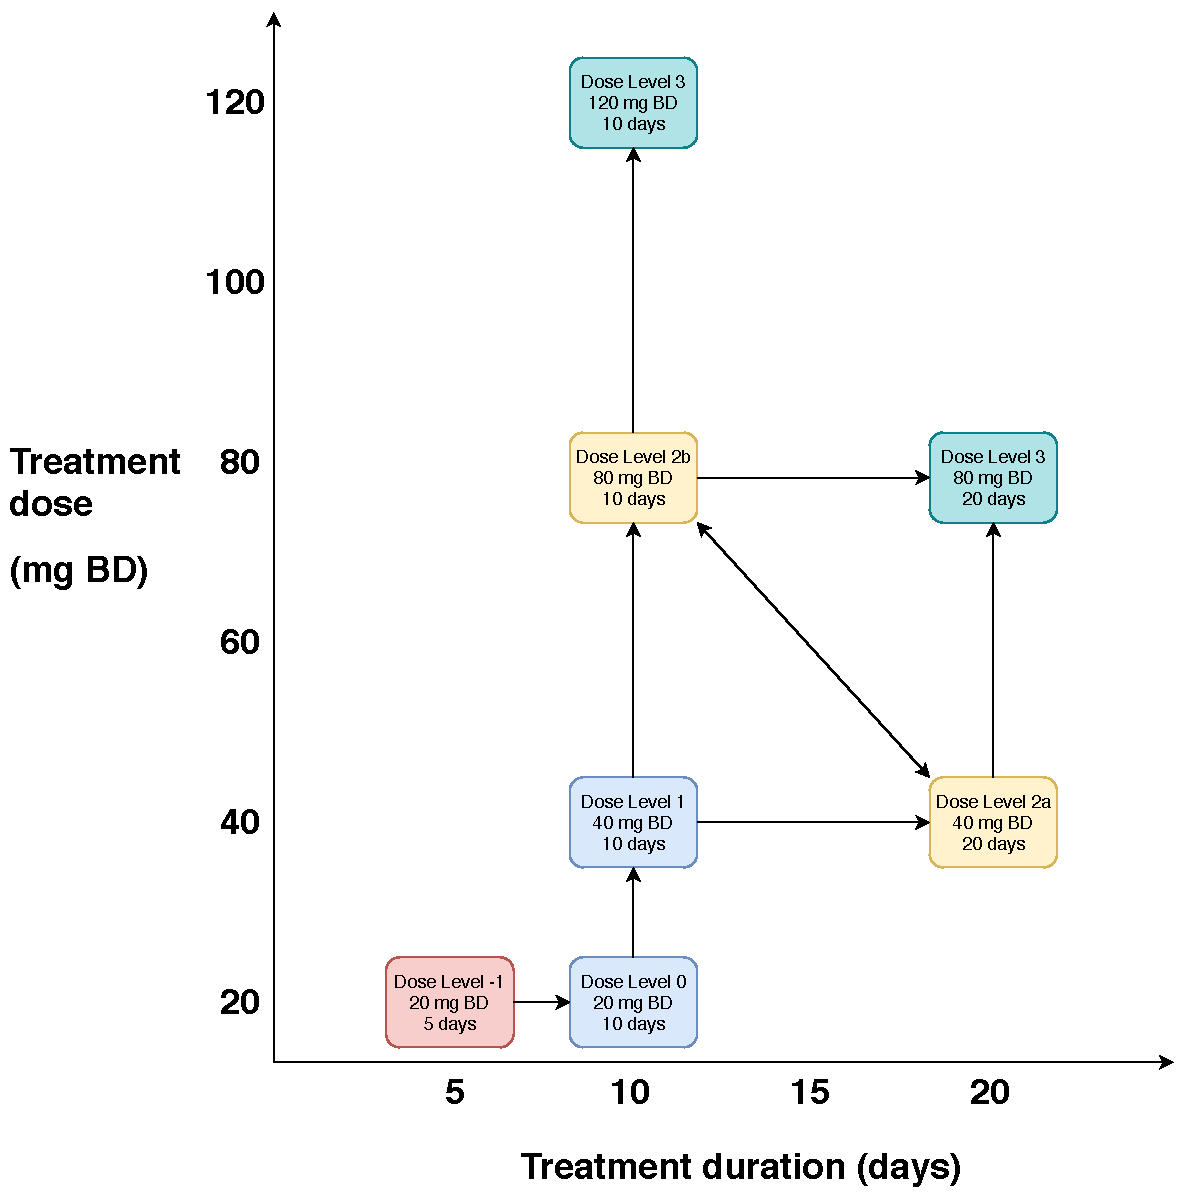
\includegraphics[width=\textwidth]{AdeptDoseCombos}
\end{figure}


\begin{itemize}
	\item Finish section 2.3
	\begin{itemize}
		\item Two-stage design of the PO-TITE-CRM 
		\item Initial dose-escalation scheme 
		\item Prior probabilities of DLT 
		\item Prior probabilities of ordering 
		\item Stopping rules 
		\item Weight function 
		\item Operating characteristics - explain why we have two sets 
	\end{itemize}
	\item Think of how to split this section up - maybe justification, trial set up 
	\item Need to think of things to extend this chapter 
	\begin{itemize}
		\item Comparisons to a normal TITE-CRM simulation 
		\item Impact of removing practical limitations from the design. For example: cohort size, sample size 
		\item Dose transition pathways in a TITE setting  
	\end{itemize}

	
\end{itemize}


%-----------------------------------
%	SUBSECTION 1
%-----------------------------------

%-----------------------------------
%	SUBSECTION 2
%-----------------------------------
